% !TeX spellcheck = cs_CZ
%================================= Kapitola: Počítačová simulace v elektrotechnice==================
\chapter{Počítačová simulace v elektrotechnice}
\minitoc

  \section{Historie}
    V roce 1971 vytvořil student „University of California“, Berkeley, USA \emph{Larry Nagel} 
    program \texttt{SPICE1} (\texttt{SPICE} = \emph{Simulation Program with Integrated Circuit 
    Emphasis}) v jazyku Fortran. Program umožňoval analýzu dějů v obvodech, obsahujících zejména 
    bipolární a
    unipolární tranzistory. O věrohodnost výsledků bylo usilováno propracovaností modelů i 
    matematických algoritmů řešení rovnic. Uživatel měl navíc  možnost roz\-ši\-řo\-vá\-ní 
    sortimentu analyzovaných součástek technikou makromodelů zakládáním tzv. \emph{pod\-ob\-vo\-dů}
    (\texttt{subcircuits}) \texttt{SPICE}. Protože program byl v podstatě volně šiřitelný, stal se 
    brzo standardním simulačním nástrojem pro elektrotechnické úlohy. Usilovně se pracovalo na jeho 
    zdokonalování.

    V roce 1975 byla představena verze \texttt{SPICE2} s podstatně vylepšenými modely i numerickými 
    algoritmy. Tato verze byla v průběhu téměř 20 let postupně zdokonalována na Berkeleyské 
    univerzitě až do dnes všeobecně známého standardu \texttt{SPICE2G.6}, který byl v r. 1983 
    zpřístupněn k volnému používání. Zdrojové texty \texttt{SPICE1} a \texttt{SPICE2} byly napsány 
    ve Fortranu. Vzhledem k zvýšenému využívání unixových pracovních stanic padlo v Berkeley 
    rozhodnutí přepsat SPICE2 do jazyka C. Tak začala vznikat verze \texttt{SPICE3}. Dnes je 
    rozšířena verze \texttt{SPICE3F.2}. Oproti SPICE2G.6 se vyznačuje řadou vylepšení, ovšem z 
    různých důvodů došlo k ztrátě zpětné kompatibility se SPICE2G.6.

    S růstem výkonnosti počítačů PC byly programy, dosud běžící na výkonných pracovních stanicích, 
    přepisovány na programy spustitelné na „PCčkách“. Tak vznikl standard \texttt{PSpice}. Dnes 
    existuje více simulačních programů, které využívají v podstatě tři ne zcela kompatibilní 
    standardy: SPICE2, SPICE3, PSPICE. Všechny lze rozdělit na tzv. „\emph{Spice-like}“ a 
    „\emph{Spice-compatible}“ simulátory.

    Označení „\emph{Spice-like}“ znamená, že simulátor je schopen generovat podobné výsledky 
    analýzy jako SPICE, avšak nemusí být schopen číst standardní vstupní soubory SPICE. Typickými 
    příklady jsou staré verze programů \texttt{Micro-Cap} nebo \texttt{TINA}, program apod. Termínem
    „\emph{Spice-compatible}“ se označují simulační programy, které dokáží číst standardní vstupní 
    soubory SPICE, provádět klasické SPICE analýzy, a generovat výsledky v standardním SPICE2G.6 
    tvaru. Ze současných programů jsou to například \texttt{PSpice}, \texttt{HSpice} (standard 
    SPICE3), \texttt{WINSpice} (standard SPICE3), \texttt{MicroCap} od verze IV, \texttt{Multisim}, 
    \texttt{LTspice} (standard SPICE3) a další.

    Kromě toho existují programy pro simulaci obvodů, které nemají s výše uvedenými skupinami 
    programů mnoho společného. Jedná se zejména o jednoúčelové programy, specializované na analýzy 
    obvodů, které nelze realizovat programy typu SPICE. Programy typu „SPICE-compatible“ jsou široce
    využívány mimo jiné proto, že umožňují neomezené rozšiřování sortimentu modelovaných součástek 
    o nové typy, jejichž modely se průběžně objevují na webu a následně i v inovovaných knihovnách 
    nových verzí programů. Na akademických pracovištích i v průmyslu je oblíbeným produktem
    OrcadPSpice.\cite[s.~10]{Biolek2}

  \section{Simulace a analýza v programu LTspice IV}
   
  \section{Příkazy pro řízení simulace}
    
    \begin{figure}[ht!]
      \centering
      \begin{tabular}{cc}
        \subfloat[ ]{\label{SPICE:fig_ltc001_Ra}
          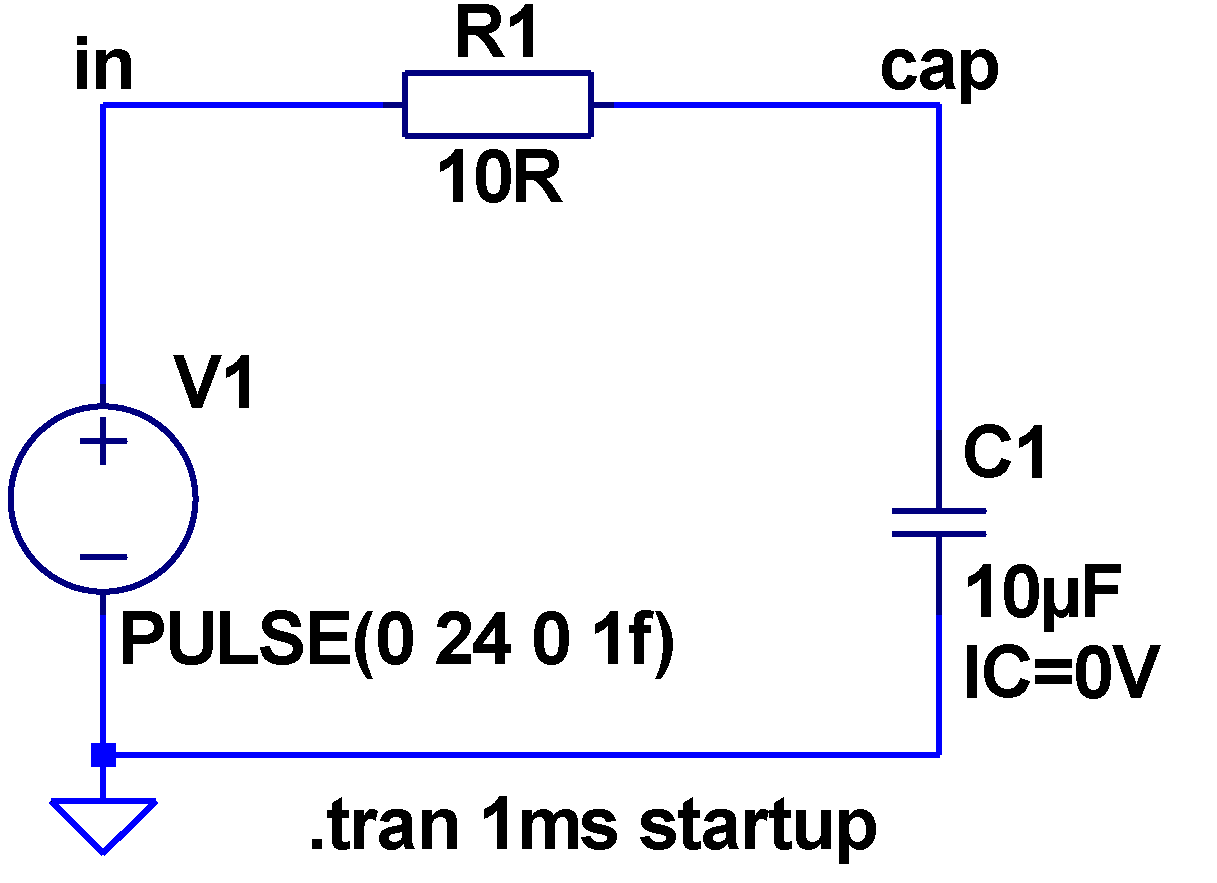
\includegraphics[width=0.45\linewidth]{../ltspice/ltc001_RC.pdf}}              &
        \subfloat[ ]{\label{SPICE:fig_ltc001_Rb} 
          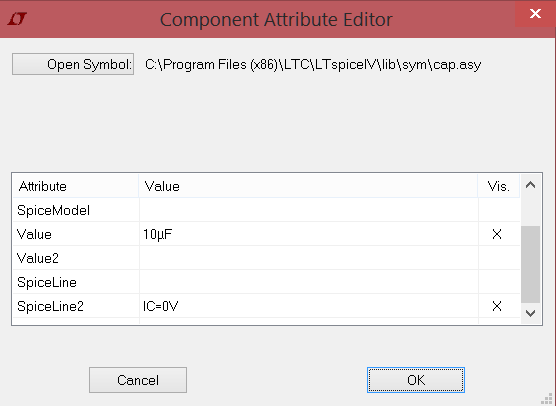
\includegraphics[width=0.45\linewidth]{../ltspice/CompAttrEditor.png}}  
      \end{tabular}
      \caption{\texttt{ltc001\_RC.asc}: Nastavení počáteční velikosti napětí na které je 
               kondenzátor nabit}
      \label{FYZ:fig_ltc001}
    \end{figure}

  \section{Osciloskopické sondy}

    \begin{figure}[ht!]
      \centering
      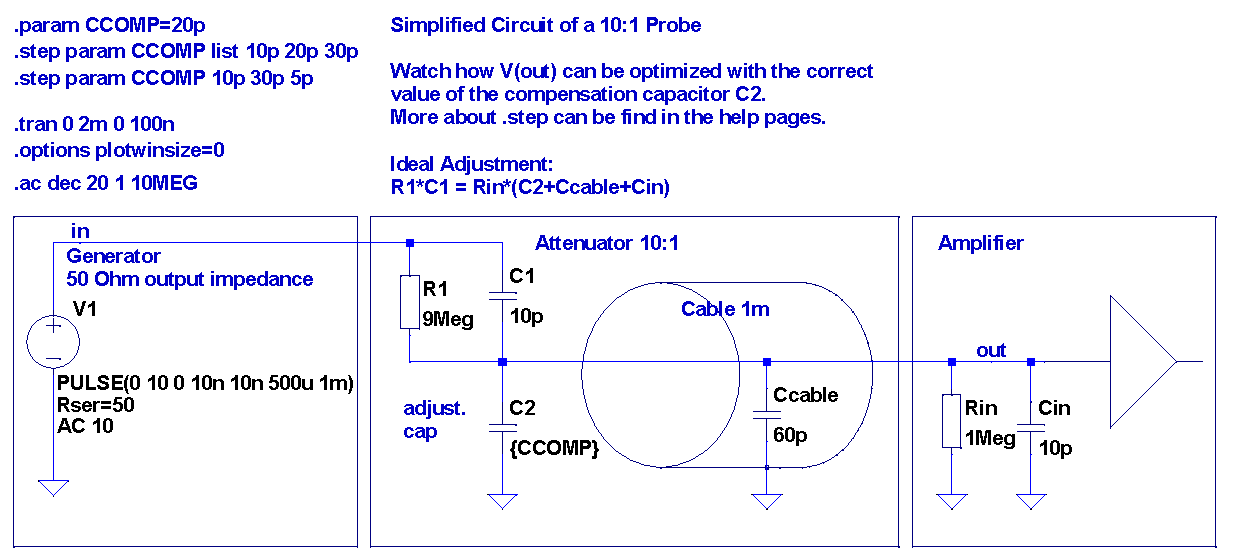
\includegraphics[width=1\linewidth]{../ltspice/ltc003_OSC_Probe_simple.pdf}
      \caption{\texttt{ltc002\_OSC\_Probe.asc}: }
      \label{SPICE:fig_ltc003_OSC}
    \end{figure}
    
    \begin{figure*}[ht!]
      \centering
      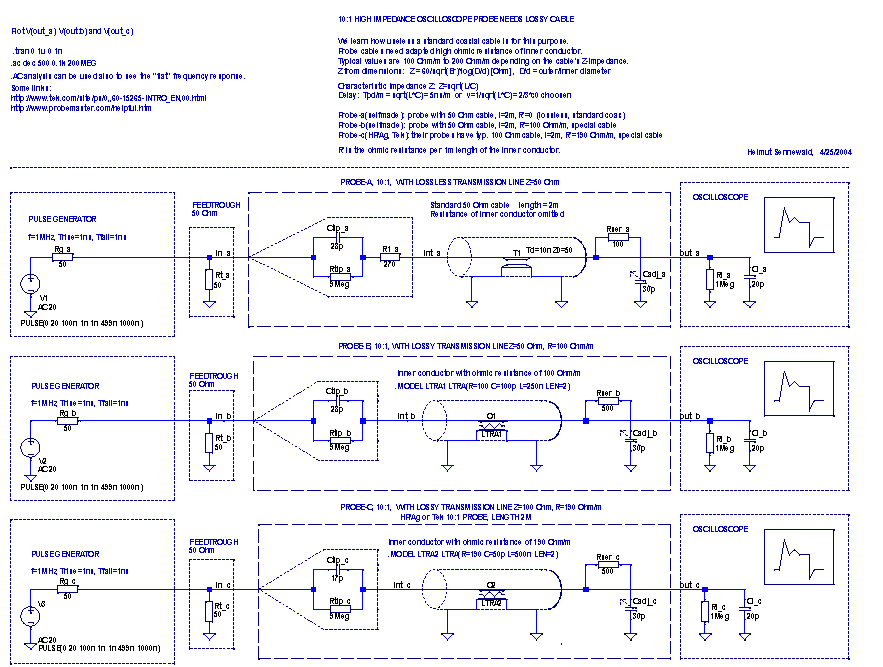
\includegraphics[width=1\linewidth]{../ltspice/ltc002_OSC_Probe.pdf}
      \caption{\texttt{ltc003\_OSC\_Probe\_simple.asc}: }
      \label{SPICE:fig_ltc002_OSC}
    \end{figure*}
    
  \section{Úvod do simulace spínaných napájecích zdrojů}
    % In the electronics world, different types of circuitries must cohabit: logic devices, analog 
    % circuits, microprocessors, and so on. Unfortunately for the designer, these circuits do not 
    % cope with a single, fixed, power supply rail: A microprocessor or a digital signal processor 
    % (DSP) will need a stable 3.3-V source or less, a front-end acquisition board will require ±15 
    % V and perhaps some logic glue around a standard 5 V. For the final board being supplied from 
    %%% a single power point, for example, the mains outlet or a battery, how is one to adapt and 
    % distribute all these different voltages to the appropriate portions? The solution consists of 
    % inserting a so-called converter to adapt the voltage distribution to the circuit needs.
    
    Ve světě elektroniky (obr. \ref{SPICE:Basso_intro}), musí různé druhy elektronických obvodů 
    vzájemně spolupracovat (logické obvody, analogové obvody, mikroprocesory, atd.). Bohužel tyto 
    obvody nepracují s jediným napájecím napětím: mikroprocesor nebo signálový procesor (DSP), bude 
    potřebovat například zdroj \SI{3.3}{\volt}, analogové obvody mohou vyžadovat symetrické nápení 
    \SI{\pm15}{\volt}. Ovšem externí napájecí zdroj je zpravidla jen jeden (např. síťové napájení 
    \SI{230}{\volt}, baterie). Vzniká tak otázka, jakým způsobem z tohoto zdroje realizovat tolik 
    napájecích úrovní. Řešení spočívá ve vložení tzv. převodníku mezi zdroj a napájený obvod, který 
    přizpůsobí napájecí napětí konkrétním požadavkům obvodu.
    
    \begin{figure}[ht!]
      \centering
      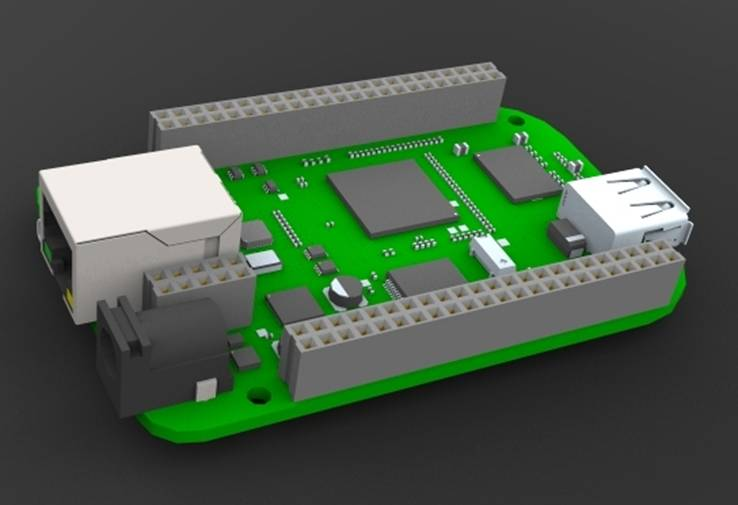
\includegraphics[width=0.6\linewidth]{beaglebone.jpg}
      \caption{Příklad plošného spoje s mnoha druhy integrovaných obvodů, vyžadující odlišné 
               napájecí úrovně}
      \label{SPICE:Basso_intro}
    \end{figure}

%---------------------------------------------------------------------------------------------------
%\printbibliography[title={Seznam literatury}, heading=subbibliography]
\addcontentsline{toc}{section}{Seznam literatury}